%-------------------------------------------------------------------------------
\documentclass[UTF8,AutoFakeBold]{resume}
%-------------------------------------------------------------------------------
\usepackage{zh_CN-Adobefonts_external}
\usepackage{linespacing_fix}
\usepackage{cite}
\usepackage{float}
\usepackage[utf8]{inputenc}
\usepackage{fontspec}
\usepackage{graphicx}
\usepackage{wrapfig} 
%-------------------------------------------------------------------------------
\usepackage{amsmath,bm}
%-------------------------------------------------------------------------------
\usepackage{booktabs}
%-------------------------------------------------------------------------------
%-------------------------------------------------------------------------------
\begin{document}
\pagenumbering{gobble}
%-------------------------------------------------------------------------------
    \begin{figure}[h]
        \flushright
        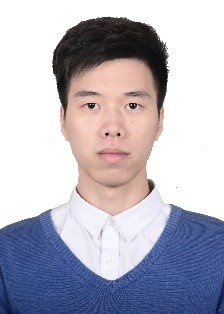
\includegraphics[height=3.5cm,width=2.5cm]{fonts/hjh.jpg}
    \end{figure}
\vspace{-0.175\linewidth}
% \vspace{-0.15\linewidth}
%-------------------------------------------------------------------------------
%%%%%%% \vspace{-0.175\linewidth}   %% 标注考研成绩 -0.175\linewidth        %%%%%%
%%%%%%% \vspace{-0.15\linewidth}    %% 隐藏考研成绩 -0.15\linewidth         %%%%%%
%-------------------------------------------------------------------------------
    \begin{minipage}[t]{0.275\textwidth}
        \centering
        \LARGE\fangsong\textbf{{黄军浩{\small{\textbullet}}个人简历}}
    \end{minipage}
%-------------------------------------------------------------------------------
%%%%%%% 取消以下注释,标注考研成绩
%-------------------------------------------------------------------------------
% \hspace{1em}
%     \begin{minipage}[t]{0.4\textwidth}\kaishu\textbf{
%         \centering
%             \begin{tabular}{ccccc}
%                 \toprule[1.5pt]
%                 思想政治理论&英语(一)&专业课一&专业课二&初试总分\\
%                 \midrule[1pt]
%                 80&80&130&130&420\\
%                 \bottomrule[1.5pt]
%             \end{tabular}
%         }
%     \end{minipage}
\vspace{3mm}
\par
% \faMapMarker \hspace{0.25em}\fangsong\textbf{广东\textbullet 珠海}
% \hspace{0.25em}{\small{\textbullet}}\hspace{0.25em}
% \makebox[0.75em][c]{\faVenus}
% \hspace{0.25em}{\small{\textbullet}}\hspace{0.25em}
% \fangsong\textbf{28岁}
\hspace{0.25em}{\small{\textbullet}}\hspace{0.25em}
\faPhone \hspace{0.25em}\textbf{(+86)18626423381}
\hspace{0.25em}{\small{\textbullet}}\hspace{0.25em}
\faEnvelope \hspace{0.25em}\textbf{\textit{jhhuang\_nuaa@126.com}}\\
\hspace{0.25em} \faChain \hspace{0.25em}\textbf{\url{https://junhaohuang.github.io}}
\par
\vspace{3mm}
%-------------------------------------------------------------------------------
%%%%%%% 取消以下注释,隐藏考研成绩
%-------------------------------------------------------------------------------
% \hspace{0.5em}\fangsong\textbf{\makebox[0.5em][c]{\faVenus}}
% \hspace{0.25em}{\small{\textbullet}}\hspace{0.25em}
% \fangsong\textbf{22岁}
% \hspace{0.25em}{\small{\textbullet}}\hspace{0.25em}
% \faPhone \textbf{\hspace{0.2em}(+86)188-8888-8888}
% \hspace{0.25em}{\small{\textbullet}}\hspace{0.25em}
% \faEnvelope \hspace{0.25em}\textbf{\textit{Oliviabcdef@163.com}}
% \vspace{12mm}

%-------------------------------------------------------------------------------
%-------------------------------------------------------------------------------
\section{\hspace{0.25em}\makebox[0.75em][c]{\faGraduationCap} \fangsong\textbf{教育背景}}
\begin{itemize}
\item \datedsubsection{\textbf{北师香港浸会大学}\qquad \qquad \textbf{密码工程方向}\qquad \quad \textbf{香港浸会大学博士}}
{\textbf{2021年 \textasciitilde \ 2025年}}
\item \datedsubsection{\textbf{南京航空航天大学}\qquad \qquad \textbf{网络空间安全}\qquad \qquad \qquad \textbf{硕士}}
{\textbf{2018年 \textasciitilde \ 2021年}}
\item \datedsubsection{\textbf{南京航空航天大学}\qquad \qquad \textbf{计算机科学与技术}\qquad \qquad \textbf{学士}}
{\textbf{2014年 \textasciitilde \ 2018年}}
\end{itemize}

\section{\hspace{0.25em}\makebox[0.75em][c]{\faGraduationCap} 
\fangsong\textbf{访问经历}}
\begin{itemize}
\item \datedsubsection{\textbf{香港城市大学}\qquad \qquad \textbf{指导老师:张泽松}\qquad \quad \textbf{}}
{\textbf{2023年7月 \textasciitilde \ 2023年12月}}
\item \datedsubsection{\textbf{武汉大学}\qquad \qquad\qquad \textbf{指导老师:何德彪}\qquad \quad \textbf{}}
{\textbf{2019年7月 \textasciitilde \ 2019年12月}}
\end{itemize}
%-------------------------------------------------------------------------------
%-------------------------------------------------------------------------------
\section{\hspace{0.25em}\makebox[0.75em][c]{\faPuzzlePiece} \fangsong\textbf{研究方向}}
\begin{itemize}
\item \textbf{密码工程,后量子密码算法,格基密码算法,取模算术}
\end{itemize}
\vspace{2mm}

\section{\hspace{0.25em}\makebox[0.75em][c]{\faGithub} \fangsong\textbf{项目经历}}
\datedsubsection{\textbf{量子安全的格密码系统软硬件协同计算平台的研究,} \textbf{国家自然科学基金}}{\textbf{2021 \textasciitilde 2023}}
\role {主要参与人}{负责Kyber和NTTRU格基密码算法在ARM Cortex-M4平台上的快速优化实现}
    \begin{itemize}
      \item \kaishu 创新性地提出了改进的Plantard模乘算法,使其具有比最优的Montgomery模乘更快、更优异的性质;
      \item \kaishu 在Cortex-M4上利用改进的Plantard模乘算法替换Montgomery算法,加速NTT/INTT计算16\%\textasciitilde 25\%。
      \item \kaishu 相关论文发表于密码工程顶会IACR CHES 2022,代码合并到pqm4。
    \end{itemize}
\datedsubsection{\textbf{格密码系统的高效及轻量级多平台实现研究,} \textbf{CCF-之江实验室联合创新基金}}{\textbf{2023 \textasciitilde 2024}}
\role {主要参与人}{负责Keccak、Kyber和Dilithium在ARMv7-M和RISC-V等平台上的快速、轻量级优化实现}
    \begin{itemize}
      \item \kaishu 进一步扩展Plantard模乘算法的输入范围$2.14$倍,提出其在32位平台M3和RISC-V上的优化实现方案;
      \item \kaishu 在ARMv7-M上进一步加速Keccak、Dilithium,Kyber和Dilithium的整体方案效率提升13\%以上;
      \item \kaishu 相关论文发表于安全顶刊IEEE TIFS 2024和密码工程顶会IACR CHES 2024,代码合并到pqm4。
    \end{itemize}
\datedsubsection{\textbf{抗量子格基隐私计算系统的异构多平台关键技术研究, } \textbf{广东省自然科学基金-面上项目}}{\textbf{2024 \textasciitilde 2026}}
\role {主要参与人}{负责基于全同态加密的隐私计算系统研究}
    \begin{itemize}
        \item \kaishu 研究基于全同态加密在决策树推理上的隐私保护技术;
        \item \kaishu 相关论文发表于CCF-B类会议ACM SIGMETRICS 2025。
    \end{itemize}

%-------------------------------------------------------------------------------
\vspace{2mm}
%-------------------------------------------------------------------------------
\section{\hspace{0.25em}\makebox[0.75em][c]{\faFlask} \fangsong\textbf{学术论文(累积合作发表15篇,代表作如下:)}}
\begin{itemize}
    \item {\textbf{Junhao Huang}, Alexandre Adomnicăi, Jipeng Zhang, Wangchen Dai, Yao Liu, Ray C. C. Cheung, \c{C}etin Kaya Ko\c{c}, Donglong Chen*. Revisiting Keccak and Dilithium Implementations on ARMv7-M. IACR CHES 2024. \textbf{CCF-B会议\& 密码工程顶会}}
    \item {\textbf{Junhao Huang}, Haosong Zhao, Jipeng Zhang, Wangchen Dai, Lu Zhou, \c{C}etin Kaya Ko\c{c}, Ray C.C. Cheung, Donglong Chen*. Yet another Improvement of Plantard Arithmetic for Faster Kyber on Low-end 32-bit IoT Devices. IEEE TIFS 2024. \textbf{CCF-A期刊\& 安全顶刊 \& \& SCI一区}}
    \item {\textbf{Junhao Huang}, Jipeng Zhang, Haosong Zhao, Zhe Liu, Ray C. C. Cheung, \c{C}etin Kaya Ko\c{c}, Donglong Chen*. Improved Plantard Arithmetic for Lattice-based Cryptography. IACR CHES 2022. \textbf{CCF-B会议\& 密码工程顶会}}
    \item {\textbf{Junhao Huang}, Zhe Liu*, Zhi Hu, Johann Großschädl. Parallel Implementation of SM2 Elliptic Curve on Intel Processor with AVX2. ACISP 2018. \textbf{CCF-C会议}}
    \item {Jipeng Zhang, \textbf{Junhao Huang}, Lirui Zhao, Donglong Chen, Çetin Kaya Koç*. ENG25519: Faster TLS 1.3 handshake using optimized X25519 and Ed25519. Usenix Security 2024. \textbf{安全四大顶会\& 杰出论文奖}}
    \item  {Jipeng Zhang, Yuxing Yan, \textbf{Junhao Huang}, Çetin Kaya Koç*. Optimized Software Implementation of Keccak, Kyber, and Dilithium on RV\{32,64\}IM\{B\}\{V\}. IACR CHES 2025. \textbf{CCF-B会议\& 密码工程顶会}}
    \item {Haosong Zhao, \textbf{Junhao Huang}, Zihang Chen, Kunxiong Zhu, Donglong Chen, Zhuoran Ji, Hongyuan Liu*}, {VESTA: A Secure and Efficient FHE-based Three-Party {V}ectorized {E}valuation {S}ystem for {T}ree {A}ggregation Models[C]}. \textit{ACM SIGMETRICS, 2025} {\bf CCF-B会议}
    \item {
		{Zewen Ye, \textbf{Junhao Huang}, Tianshun Huang, Yudan Bai, Jinze Li, Hao Zhang, Guangyan Li, Donglong Chen, Ray CC Cheung, Kejie Huang*}, {PQNTRU: Acceleration of NTRU-based Schemes via Customized Post-Quantum Processor[J]}. \textit{IEEE Transactions on Computers, 2025} {\bf CCF-A期刊\& SCI二区}
	}
    \item {Jipeng Zhang, \textbf{Junhao Huang}, Zhe Liu*, Sujoy Sinha Roy. Time-memory Trade-offs for Saber on Memory-constrained RISC-V. IEEE TC 2022. \textbf{CCF-A期刊\& SCI二区}}
   
    \item {Xinyi Ji, Jiankuo Dong, \textbf{Junhao Huang}, Zhijian Yuan, Wangchen Dai, Fu Xiao, Jingqiang Lin. ECO-CRYSTALS: Efficient Cryptography CRYSTALS on Standard RISC-V ISA. IEEE TC 2024. \textbf{CCF-A期刊\& SCI二区}}
\end{itemize}

\vspace{2mm}
%-------------------------------------------------------------------------------
%-------------------------------------------------------------------------------
\section{\hspace{0.25em}\makebox[0.75em][c]{\faTrophy} \fangsong\textbf{荣誉奖项}}
    \vspace{0.1em}
    \begin{itemize}
        \item \datedline{\kaishu 2024年广东省计算机学会优秀论文奖\qquad \qquad \textbf{一等奖}}{\textbf{2024年12月}}
        \item \datedline{\kaishu Usenix Security 2024\qquad \qquad\qquad\qquad\qquad\quad  \textbf{杰出论文奖}}{\textbf{2024年8月}}
        \item \datedline{\kaishu 2023年广东网络空间安全优秀论文奖\qquad \qquad \textbf{三等奖}}{\textbf{2023年5月}}
        % \item \datedline{\kaishu 研究生学业奖学金\qquad\qquad\qquad\qquad\quad \textbf{一等奖}}{\textbf{2018年10月}}
    \end{itemize}
\vspace{2mm}
%-------------------------------------------------------------------------------
%-------------------------------------------------------------------------------
% \section{\hspace{0.25em}\makebox[0.75em][c]{\faPuzzlePiece} \fangsong\textbf{专业技能}}
% \noindent

% \begin{itemize}
%     \item \kaishu\textbf{编程语言}: C, ARMv7-M汇编, RISC-V汇编, Intel AVX2汇编, Python
%     \item \kaishu\textbf{英语能力}: CET-4(597), CET-6(512), IELTS(7.0)
% \end{itemize}

% \vspace{2mm}
%-------------------------------------------------------------------------------
%-------------------------------------------------------------------------------
\section{\hspace{0.25em}\makebox[0.75em][c]{\faUsers} \fangsong\textbf{学术推荐人}}
\vspace{0.1em}
    \begin{itemize}
        \item \kaishu 陈东龙(副教授,副系主任,导师),北师香港浸会大学,donglongchen@uic.edu.cn
        \item \kaishu 张泽松(教授,副校长,访问学者导师),香港城市大学,r.cheung@cityu.edu.hk
        \item \kaishu Çetin Kaya Koç(教授,IEEE Life Fellow,CHES发起人之一),加州大学圣巴巴拉分校,cetinkoc@ucsb.edu
    \end{itemize}
%-------------------------------------------------------------------------------
%-------------------------------------------------------------------------------
\end{document}